%% storify worked example, built on scaling_vault, question "Does more data beat a
%% better model?" and its three experiments. Edit THIS file. Run
%% `python3 build_story.py` to write story.tex, then `latexmk -pdf story.tex`.
%% Never edit story.tex by hand: the build overwrites it.
%%
%% numbers   every measured number is a macro the build defines in the data slot below,
%%           read from results/h1, results/h2 and results/h3 (metrics.json).
%% typed     \lit{95} (the confidence level) and \lit{2.0} (the pre-registered
%%           threshold, in points); nothing else.
\documentclass[pdflatex,sn-mathphys-num]{sn-jnl}

% crux-sources: __SOURCES__

\usepackage{graphicx}
\usepackage{amsmath}
\usepackage{booktabs}
\usepackage{xcolor}
\usepackage{tikz}
\usetikzlibrary{positioning,arrows.meta,calc}
\usepackage{pgfplots}
\pgfplotsset{compat=1.18}
\usepackage{pgfplotstable}

% A design constant typed in prose, e.g. \lit{95}. It renders its argument unchanged.
\newcommand{\lit}[1]{#1}

% One colour per arm and one per budget, defined once and reused in every figure.
\definecolor{dataarm}{HTML}{3F7D7A}
\definecolor{modelarm}{HTML}{B5462E}
\definecolor{owncost}{HTML}{3F7D7A}
\definecolor{eqcompute}{HTML}{B5462E}

% The build replaces the next line with the number macros and the chart tables.
% __DATA__

\raggedbottom

\begin{document}

\title[More data or a better model]{More data beats a better model only when it is also given more compute}

\author{\fnm{Mehdi} \sur{Foroozandeh}}
\affil{\orgname{Scaling study, private draft, \today}}

\abstract{We asked whether doubling the training set buys more accuracy than a
higher-capacity model, once both choices cost the same. At each arm's own cost, twice the
data won by \dFirstOwn{} points on the first task (\lit{95}\% confidence interval
\loFirstOwn{} to \hiFirstOwn{}). Matched on training compute, the same comparison reversed
to \dFirstEqc{} points, and on a harder task the data arm never led. The data advantage we
first saw was mostly a budget advantage; the study covers two tasks and one pair of model
families.}

\keywords{scaling, training data, model capacity, compute budget, controlled comparison}

\maketitle

\section{Motivation and background}\label{sec:motivation}

Test error falls as a power law in both training-set size and model size
\cite{kaplan2020}. Which lever pays more is therefore an empirical question about where a
project sits, not a general fact. The usual comparison runs each choice at the settings
that suit it. Doubling the training set then also doubles the training compute, so data
size is confounded with compute (two causes change together, so their effects cannot be
separated). A win for the data-rich model is then a win for more data and for more compute
at once.

The field has paid for this confound before. Compute-optimal training showed that a
generation of large language models had been built far larger than their budgets
justified; a smaller model trained on more data won at the same compute
\cite{hoffmann2022}. Our question is the controlled version: if we can afford either twice
the data or a better model, which one buys more accuracy when both spend the same compute?

\section{Methods}\label{sec:methods}

Figure~\ref{fig:design} shows the design. The data arm is a smaller convolutional network
\cite{he2015} trained on \nTrainData{} examples. The model arm is a larger vision
transformer (an attention-based image model) \cite{dosovitskiy2020} trained on the
original \nTrainBase{} examples. Both arms share one fine-tuning protocol (the fixed recipe
that adapts a pretrained model to the task). Each arm runs \nSeeds{} seeds (independent
random restarts of training) and is scored on \nHeldout{} held-out examples (never used in
training).

Every comparison was run twice: once with each arm at its own cost, and once at equal
training compute, counted in FLOPs (floating-point operations). To match compute, the data
arm's training is shortened, never extended, so no arm exceeds its budget. The model
families, the protocol, the seed count and the two budgets were pre-registered (fixed in
writing before any run), with a threshold of a gain of at least \lit{2.0} points on the
first task.

The outcome is the accuracy difference, data arm minus model arm, in percentage points.
Each difference carries its \lit{95}\% confidence interval (range that holds the true
difference in \lit{95}\% of repeats) across seeds. A difference is statistically
significant (unlikely to arise from chance alone) only when its interval excludes zero.

\begin{figure}[t]
\centering
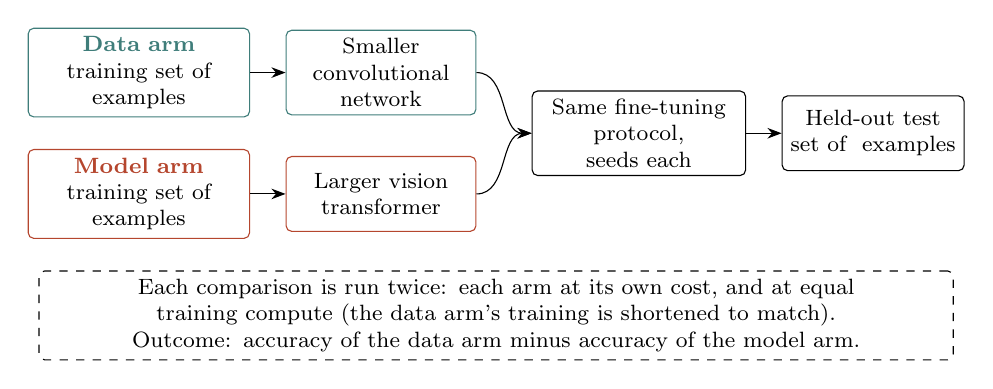
\begin{tikzpicture}[
    box/.style={draw, rounded corners=2pt, align=center, font=\footnotesize,
      minimum height=0.95cm, inner sep=3pt},
    >={Stealth[length=1.8mm]}]
  % the two arms
  \node[box, draw=dataarm, text width=2.6cm] (dd)
    {\textbf{\color{dataarm}Data arm}\\ training set of\\ \nTrainData{} examples};
  \node[box, draw=dataarm, text width=2.2cm, right=0.45cm of dd] (dm)
    {Smaller\\ convolutional network};
  \node[box, draw=modelarm, text width=2.6cm, below=0.4cm of dd] (md)
    {\textbf{\color{modelarm}Model arm}\\ training set of\\ \nTrainBase{} examples};
  \node[box, draw=modelarm, text width=2.2cm, right=0.45cm of md] (mm)
    {Larger vision\\ transformer};
  \draw[->] (dd) -- (dm);
  \draw[->] (md) -- (mm);
  % shared fine-tuning and scoring
  \node[box, text width=2.5cm, right=0.7cm of $(dm.east)!0.5!(mm.east)$] (ft)
    {Same fine-tuning\\ protocol,\\ \nSeeds{} seeds each};
  \node[box, text width=2.1cm, right=0.45cm of ft] (ev)
    {Held-out test set of \nHeldout{} examples};
  \draw[->] (dm.east) to[out=0, in=180] (ft.west);
  \draw[->] (mm.east) to[out=0, in=180] (ft.west);
  \draw[->] (ft) -- (ev);
  % the two budgets
  \node[box, dashed, text width=11.4cm, below=0.4cm of $(md.south west)!0.5!(ev.east |- md.south)$]
    (bud) {Each comparison is run twice: each arm at its own cost, and at equal training
    compute (the data arm's training is shortened to match).\\
    Outcome: accuracy of the data arm minus accuracy of the model arm.};
\end{tikzpicture}
\caption{Study design. The two arms differ only in training-set size and model capacity;
the fine-tuning protocol, the seeds and the test set are shared.}\label{fig:design}
\end{figure}

\section{Results and discussion}\label{sec:results}

\paragraph{At its own cost, more data wins.} On the first task the data arm reached
\accDataFirstOwn{}\% accuracy against \accModelFirstOwn{}\% for the model arm, a
difference of \dFirstOwn{} points (\lit{95}\% confidence interval \loFirstOwn{} to
\hiFirstOwn{}; Fig.~\ref{fig:results}a). It cleared the pre-registered threshold. The gain
replicated in an independent rerun (\dRepOwn{}, \loRepOwn{} to \hiRepOwn{}) and held on a
second task (\dSecondOwn{}, \loSecondOwn{} to \hiSecondOwn{}). This is the comparison most
papers report, and it does not hold compute fixed.

\paragraph{At equal compute, the advantage reverses.} Once the data arm's training was
shortened to the model arm's budget, the first-task difference fell to \dFirstEqc{} points
(\loFirstEqc{} to \hiFirstEqc{}), a swing of \swingFirst{} points. The model arm improved
to \accModelFirstEqc{}\% while the data arm fell to \accDataFirstEqc{}\%
(Fig.~\ref{fig:results}b). Most of the data advantage was therefore extra compute, not
extra data. One caveat applies: shortening training is one way to match compute, and
growing the model arm is another that we did not test.

\paragraph{On a harder task, the data arm never leads.} At its own cost the data arm scored
\accDataHardOwn{}\% against \accModelHardOwn{}\%, a difference of \dHardOwn{} points
(\loHardOwn{} to \hiHardOwn{}). This difference is not statistically significant, because
its interval includes zero; it is a null result, not a small loss. At equal compute the
difference was \dHardEqc{} points (\loHardEqc{} to \hiHardEqc{}), clearly negative. We keep
this negative result: it rules out reading the first task as the general case. A plausible
reason is inductive bias (built-in assumptions that help when data is scarce), which
favours convolutional networks on easier tasks.

Across all \nCompared{} differences, \nSig{} are statistically significant. Every significant
positive difference comes from the own-cost budget; every comparison at equal compute
favours the model arm.

\begin{figure}[t]
\centering
\begin{tikzpicture}
\begin{axis}[name=diffs, width=0.58\linewidth, height=5cm,
    title={\small (a) Accuracy difference, data arm minus model arm},
    xlabel={Difference (percentage points)}, xmin=-7.5, xmax=5.5,
    ymin=0.3, ymax=7.7, ytick={1,2,4,5,6,7}, ytick style={draw=none},
    yticklabels={Harder task, First task, Harder task, Second task, {First task, rerun},
      First task},
    tick label style={font=\scriptsize}, label style={font=\footnotesize},
    extra x ticks={0}, extra x tick labels={},
    extra x tick style={grid=major, grid style={gray, thin}},
    legend style={font=\scriptsize, at={(1.04,0.5)}, anchor=west, draw=none},
    legend cell align=left]
  \addplot[only marks, mark=*, mark size=1.8pt, color=owncost,
      error bars/.cd, x dir=both, x explicit, error bar style={line width=0.8pt}]
    table[x=d, y=y, x error plus=ep, x error minus=em]{\tblOwn};
  \addlegendentry{Each arm at its own cost}
  \addplot[only marks, mark=square*, mark size=1.8pt, color=eqcompute,
      error bars/.cd, x dir=both, x explicit, error bar style={line width=0.8pt}]
    table[x=d, y=y, x error plus=ep, x error minus=em]{\tblEqc};
  \addlegendentry{Equal training compute}
\end{axis}
\begin{axis}[at={(diffs.south west)}, anchor=north west, yshift=-2.1cm,
    width=0.58\linewidth, height=4.4cm,
    title={\small (b) Accuracy of each arm},
    ybar, bar width=9pt, ymin=0, ymax=60, ylabel={Accuracy (\%)},
    xtick={0,1,2}, xticklabels={{First task,\\own cost}, {First task,\\equal compute},
      {Harder task,\\own cost}},
    xticklabel style={align=center}, xtick style={draw=none},
    enlarge x limits=0.22,
    tick label style={font=\scriptsize}, label style={font=\footnotesize},
    legend style={font=\scriptsize, at={(1.04,0.5)}, anchor=west, draw=none},
    legend cell align=left, area legend]
  \addplot[fill=dataarm, draw=none] table[x=x, y=data]{\tblAcc};
  \addlegendentry{Data arm}
  \addplot[fill=modelarm, draw=none] table[x=x, y=model]{\tblAcc};
  \addlegendentry{Model arm}
\end{axis}
\end{tikzpicture}
\caption{(a) Accuracy difference between the arms, data arm minus model arm. Each horizontal line is
the \lit{95}\% confidence interval across seeds; an interval that crosses the zero line is
not statistically significant. Circles are each arm at its own cost; squares are equal
training compute. (b) Mean accuracy of each arm where the result files hold both values.
The uncertainty of each comparison is the interval of its difference in panel (a).}
\label{fig:results}
\end{figure}

\section{Conclusion}\label{sec:conclusion}

More data beats a better model only while it also gets more compute. At each arm's own
cost twice the data won and the result replicated; at equal compute it lost on both tasks,
and on the harder task it never led. The limitations are two tasks, one pair of model
families, and one way of matching compute. The second task was not run at equal compute.

Three next steps are open, listed without ranking:
\begin{itemize}
\item \textbf{Find the data floor.} Measure how little data still matches the better model.
This is cheap, and it shows where the accuracy curve bends.
\item \textbf{Match compute a second way.} Grow the model arm instead of shortening the data
arm. This costs a moderate amount, and it tests the matching rule itself.
\item \textbf{Repeat on data from another source.} This is the most costly option, and it
tests whether any of these results transfer.
\end{itemize}

\backmatter

\bibliography{references}

\end{document}
